% figure: 现控5-32-观测器反馈状态框图.png
% Observer-based feedback, with the same actual input u sent to both blocks.
\documentclass[border=10pt]{standalone}
\usepackage{fontspec}
\setmainfont{Cambria}
\usepackage{unicode-math}
\setmathfont{Cambria Math}
\usepackage{tikz}
\usetikzlibrary{arrows.meta,calc}
\definecolor{ink}{HTML}{1E2228}
\definecolor{paperblue}{HTML}{E8EFF8}
\begin{document}
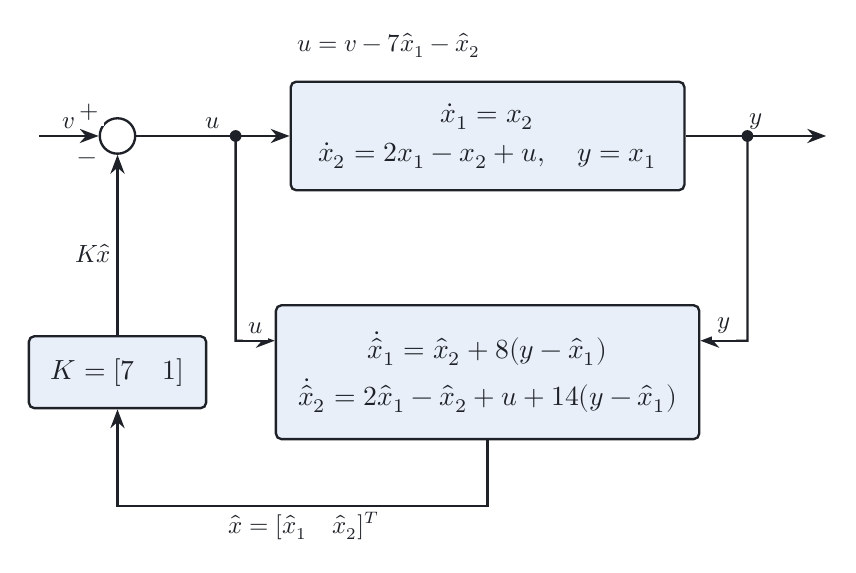
\begin{tikzpicture}[
  >=Stealth,draw=ink,text=ink,line width=0.85pt,
  block/.style={draw,fill=paperblue,rounded corners=2pt,align=center,inner sep=8pt},
  lab/.style={font=\small,fill=white,inner sep=2pt},
  dot/.style={circle,fill=ink,inner sep=1.5pt}
]
\node[draw,circle,minimum size=0.45cm,inner sep=0pt] (sum) at (0,0) {};
\node[block,minimum width=5cm,minimum height=1.15cm] (plant) at (4.7,0)
  {$\dot x_1=x_2$\\[2pt]$\dot x_2=2x_1-x_2+u,\quad y=x_1$};
\node[block,minimum width=5cm,minimum height=1.7cm] (obs) at (4.7,-3)
  {$\dot{\hat x}_1=\hat x_2+8(y-\hat x_1)$\\[4pt]
   $\dot{\hat x}_2=2\hat x_1-\hat x_2+u+14(y-\hat x_1)$};
\node[block,minimum width=1.6cm,minimum height=0.85cm] (gain) at (0,-3) {$K=[7\quad1]$};
\coordinate (u) at (1.5,0);
\coordinate (y) at (8,0);
\draw[->] (-1,0) -- node[lab,above] {$v$} (sum.west);
\draw[->] (sum.east) -- node[lab,above,pos=0.5] {$u$} (plant.west);
\draw[->] (plant.east) -- node[lab,above] {$y$} (9,0);
\node[dot] at (u) {};
\node[dot] at (y) {};
\draw[->] (u) -- (1.5,-2.6) -- node[lab,above] {$u$} ($(obs.west)+(0,0.4)$);
\draw[->] (y) -- (8,-2.6) -- node[lab,above] {$y$} ($(obs.east)+(0,0.4)$);
\draw[->] (obs.south) -- (4.7,-4.7) -- node[lab,below] {$\hat x=[\hat x_1\quad\hat x_2]^T$} (0,-4.7) -- (gain.south);
\draw[->] (gain.north) -- node[lab,left,pos=0.45] {$K\hat x$} (sum.south);
\node[lab] at (-0.36,0.3) {$+$};
\node[lab] at (-0.38,-0.32) {$-$};
\node[lab,anchor=west] at (2.2,1.15) {$u=v-7\hat x_1-\hat x_2$};
\end{tikzpicture}
\end{document}
